\documentclass[10pt]{beamer}

\usepackage[utf8]{inputenc}
\usepackage[spanish, es-tabla]{babel}

\usetheme{metropolis}
\usepackage{appendixnumberbeamer}

\usepackage{booktabs}
\usepackage[scale=2]{ccicons}

\usepackage{pgfplots}
\usepgfplotslibrary{dateplot}

\usepackage{caption}
\usepackage{subcaption}

\usepackage{graphicx}

\usepackage{amsmath}
\usepackage{amsfonts}
\usepackage{amssymb}
\usepackage{amsthm}
\usepackage{esvect}

\usepackage{xspace}
\newcommand{\themename}{\textbf{\textsc{metropolis}}\xspace}

\title{Análisis Factorial}
\author{Ignacio Aguilera Martos}
\date{\today}
\institute{Estadística Multivariante \\ \href{https://github.com/nacheteam/Analisis-Factorial}{Link: \underline{Documentos LaTeX en GitHub}}}

\begin{document}

\maketitle

\begin{frame}[fragile]{Contenidos}
  \setbeamertemplate{section in toc}[sections numbered]
  \tableofcontents[hideallsubsections]
\end{frame}

%%%%%%%%%%%%%%%%%%%%%%%%%%%%%%%%%%%%%%%%%%%%%%%%%%%%%%%%%%%%%%%%%%%%%%%%%%%%%%%%%%%%%%%%%%%%%
%%                          Explicación teórica del modelo                                 %%
%%%%%%%%%%%%%%%%%%%%%%%%%%%%%%%%%%%%%%%%%%%%%%%%%%%%%%%%%%%%%%%%%%%%%%%%%%%%%%%%%%%%%%%%%%%%%

\section{Explicación teórica del modelo}

\begin{frame}[fragile]{Modelo}
	\vspace{10px}
	\metroset{block=fill}
	\begin{alertblock}{Idea de AF}
		El objetivo de este modelo es, dada una matriz de covarianzas, ser capaz de explicar esta matriz a partir de factores no observados llamados factores comunes, de forma que se pueda explicar la matriz con un número menor de variables que en un punto inicial.
	\end{alertblock}
	De esta forma matricialmente si tenemos n observaciones de dimensión p tendríamos una matriz
	$F=
	\begin{pmatrix}
	F_{11} & ... & F_{1n} \\
	... & ... & ... \\
	F_{k1} & ... & F_{kn}
	\end{pmatrix}
	$ de factores y 
	$L=
	\begin{pmatrix}
	l_{11} & ... & l_{1k} \\
	... & ... & ... \\
	l_{p1} & ... & l_{pk}	
	\end{pmatrix}
	$ una matriz de coeficientes de forma que $x-\mu = LF + \epsilon$ donde $\epsilon$ es un vector de errores.
\end{frame}

\begin{frame}[fragile]{Tipos de Análisis Factorial}
\vspace{10px}
\metroset{block=fill}
\begin{block}{Tipos}
	\begin{itemize}
		\item EFA (Exploratory Factor Analysis): se usa para identificar relaciones complejas entre conceptos o grupos de conceptos.
		\item CFA (Confirmatory Factor Analsysis): está dirigida a la confirmación de factores que ya se presuponen importantes para explicar la matriz de correlación o covarianza.
	\end{itemize}
\end{block}
\end{frame}

\begin{frame}[fragile]{EFA}
\vspace{10px}
\metroset{block=fill}
\begin{block}{Procesos de ajuste}
	\begin{itemize}
		\item Máxima verosimilitud: es una buena opción cuando los datos se distribuyen según una normal. Se intenta que el modelo de los factores obtenidos tenga máxima verosimilitud.
		\item Factorización en el eje principal: la intención es ir obteniendo factores de forma que el primero tenga la varianza lo más próxima al objetivo, el segundo factor la segunda varianza más próxima a la varianza objetivo, etc. Maximiza la fórmula del modelo.
	\end{itemize}
\end{block}
\end{frame}

\begin{frame}[fragile]{EFA}
	La rotación de factores se emplea para obtener la estructura de factores más simple escogiendo una orientación de los mismos.
	\vspace{10px}
	\metroset{block=fill}
	\begin{block}{Rotación de factores}
		\begin{itemize}
			\item Ortogonal: implica que los factores estén incorrelados y busca la estructura más simple.
			\item Oblicua: permite que los factores estén correlados y busca la estructura más simple.
		\end{itemize}
	\end{block}
\end{frame}


\begin{frame}[fragile]{EFA}
No sólo tenemos que estudiar la generación de los factores, si no también cuántos factores debemos escoger.
\vspace{10px}
\metroset{block=fill}
\begin{block}{Métodos para escoger el número de factores}
	\begin{itemize}
		\item Regla de Kaiser: tomamos los valores propios de la matriz de entrada y comprobamos cuántos de ellos son mayores que 1. Este es el número de factores a tomar. En caso de no haberlo se toma un factor.
		\item Criterio de la gráfica de Cattell's: obtenemos los valores propios de la matriz de entrada y los pintamos de mayor a menor. Analizamos el cambio entre los valores propios y donde se produzca el último cambio brusco contamos el número de valores propios hasta él. Este es el número de factores. Es un método subjetivo y ampliamente criticado.
	\end{itemize}
\end{block}
\end{frame}

\begin{frame}[fragile]{EFA}
\vspace{10px}
\metroset{block=fill}
\begin{block}{Métodos para escoger el número de factores}
	\begin{itemize}
		\item VSS (Very Simple Structure): este procedimiento toma un modelo simplificado del problema e intenta ver para qué número de factores los valores obtenidos se acercan más a los que deberían ser.
		\item Comparación de modelos: intentan obtener una medida de cómo de bueno y complejo es el modelo creado con un número de factores dado, de forma que se intenta maximizar el resultado y minimizar la complejidad.
		\item OC (Optimal Coordinate): intenta eliminar la subjetividad del método de Cattell. Se calculan los gradientes en la misma gráfica de dicho método y se comprueba dónde hay un cambio más abrupto. Esto delimita el número de factores.
		\item AF (Acceleration Factor): persigue el mismo objetivo que el método anterior, salvo que en este caso se realiza el cálculo con la pendiente de la curva asociada.
	\end{itemize}
\end{block}
\end{frame}

\begin{frame}[fragile]{EFA}
\vspace{10px}
\metroset{block=fill}
\begin{block}{Métodos para escoger el número de factores}
	\begin{itemize}
		\item MAP (Minimum Average Partial) test: se realiza, desde k=1 hasta el número de variables menos 1 un análisis PCA del modelo con k número de factores. Se estudia cómo se comporta dicho modelo con k factores y se toma el valor de k para el cual se ha obtenido el mejor resultado.
		\item PA (Parallel Analysis): tomamos la misma gráfica que en el método de Cattell y generamos aleatoriamente un conjunto de valores. Estos valores representan los valores medios de los valores propios de matrices aleatorias con el mismo número de variables y datos que la original. Hallamos la media para estos valores y tomamos como número de factores el de los que superen este valor medio. Se puede ver como un refinamiento de la regla de Kaiser ajustando la cota.
	\end{itemize}
\end{block}
\end{frame}

\begin{frame}[fragile]{EFA}
\vspace{10px}
\metroset{block=fill}
\begin{block}{Métodos para escoger el número de factores}
	\begin{itemize}
		\item Comparación de datos: se realiza una comparación entre modelos con una separación en factores ya conocida como correcta comparando los valores propios de la matriz y los factores escogidos en cada caso. Se toma el número de factores del modelo cuyos valores propios se parezcan más a los del caso que estamos analizando.
		\item Convergencia de múltiples tests: esta estrategia busca de forma empírica el mejor número de factores analizando la convergencia del modelo.
	\end{itemize}
\end{block}
\end{frame}

\begin{frame}[fragile]{CFA}
	El objetivo de CFA es, dada una hipótesis sobre el número de factores, si los factores están o no correlados y qué variables se relacionan con cada factor. Es por esto que EFA y CFA se usan en contextos muy diferentes aún siendo los dos tipos del mismo método.
\end{frame}

\begin{frame}[fragile]{CFA}
\vspace{10px}
\metroset{block=fill}
\begin{block}{Métodos para evaluar la hipótesis}
	\begin{itemize}
		\item Ajuste absoluto: consiste en obtener una medida absoluta de cómo de ajusta el modelo hipotético a los valores proporcionados.
		\item Ajuste relativo: obtiene una medida comparativa de cómo funciona con respecto a un modelo llamado base. Este modelo es fijo y nos sirve para obtener una valoración absoluta del mismo muy mala, de forma que con el ajuste relativo obtenemos una medida de cuánto se acerca la medida de nuestra hipótesis a la de este modelo con mal ajuste.
	\end{itemize}
\end{block}
\end{frame}

\begin{frame}[fragile]{CFA}
\vspace{10px}
\metroset{block=fill}
\begin{block}{Medidas de ajuste absoluto}
	\begin{itemize}
		\item Test chi-cuadrado: nos da la diferencia entre la matriz de covarianza observada y predicha con el modelo hipotético. Cuanto más cercano sea el valor a cero mejor es el ajuste.
		\item Aproximación según la raíz cuadrada del error: se obtiene un valor entre 0 y 1 que mide el error del modelo con respecto a la observación. Cuanto más cercano sea el valor a 0 mejor es el ajuste.
		\item Raíz cuadrada de la media de los residuos al cuadrado y raíz cuadrada de la media de los residuos estandarizados al cuadrado: no sólo estudiamos los residuos si no que además estandarizamos las variables para que los valores obtenidos sean comparables. El rango de valores está entre 0 y 1 siendo 0 la mejor medida. Normalmente cuando tenemos una puntuación de menos de 0.08 decimos que el modelo es robusto
	\end{itemize}
\end{block}
\end{frame}

\begin{frame}[fragile]{CFA}
\vspace{10px}
\metroset{block=fill}
\begin{block}{Medidas de ajuste absoluto}
	\begin{itemize}
		\item Índice de bondad del ajuste e índice de bondad del ajuste equilibrado: son medidas del ajuste del modelo y la matriz de covarianza observada. El índice equilibrado pondera el valor de ajuste en la matriz de covarianza para cada factor en función de cuántas variables explique. Los valores que arroja están entre 0 y 1 siendo a partir de 0.9 un buen modelo.
	\end{itemize}
\end{block}
\end{frame}

\begin{frame}[fragile]{CFA}
\vspace{10px}
\metroset{block=fill}
\begin{block}{Medidas de ajuste relativo}
	\begin{itemize}
		\item Índice de ajuste normado e índice de ajuste no normado: el índice normado analiza las discrepancias entre el valor de la chi-cuadrado con los del modelo y los del modelo base. El problema de este índice es que no es insesgado, lo cual es corregido por el índice de ajuste no normado el cual se mueve entre 0 y 1, siendo valores mayores o iguales a 0.95 indicativos de un buen modelo.
		\item Índice de ajuste comparativo: el anterior índice normado tiene una alta sensibilidad a la dimensión de la muestra tomada, de forma que este índice se plante extender la idea sin este problema- Compara el ajuste del modelo con un modelo base independiente. Los valores de este índice están ente 0 y 1 siendo necesarios valores mayores o iguales a 0.9 para considerar a la hipótesis un buen modelo.
	\end{itemize}
\end{block}
\end{frame}

\begin{frame}[fragile]{PCA y FA}
¿Cuál es la diferencia entonces con PCA?
\vspace{10px}
\metroset{block=fill}
\begin{alertblock}{Diferencia entre PCA y AF}
	\begin{itemize}
		\item PCA se puede emplear como un posible método de ajuste en la primera fase de EFA en la que extraemos los factores. Tras esto viene la fase de rotación de los mismos para escoger una orientación.
		\item Precisamente, por la carencia de la rotación, PCA no obtiene unos factores únicos, mientras que EFA sí. 
		\item Con AF queremos explicar el modelo en base a factores no observados, con PCA queremos explicar el modelo con menos variables.
	\end{itemize}
\end{alertblock}
\end{frame}

%%%%%%%%%%%%%%%%%%%%%%%%%%%%%%%%%%%%%%%%%%%%%%%%%%%%%%%%%%%%%%%%%%%%%%%%%%%%%%%%%%%%%%%%%%%%%
%%                         Explicación del ejemplo y uso en R                              %%
%%%%%%%%%%%%%%%%%%%%%%%%%%%%%%%%%%%%%%%%%%%%%%%%%%%%%%%%%%%%%%%%%%%%%%%%%%%%%%%%%%%%%%%%%%%%%

\section{Explicación del ejemplo en R}

\begin{frame}[fragile]{Instalación}
	\vspace{10px}
	\metroset{block=fill}
	\begin{block}{Paquetes a instalar}
		\begin{itemize}
			\item install.packages(``psych''): implementa Análisis Factorial Exploratorio
			\item install.packages(``GPArotation''): implementa la Rotación de Factores
			\item install.packages(``cfa''): implementa Análisis Factorial Confirmatorio
			\item install.packages(``lavaan''): implementa la sintaxis de especificación del modelo para cfa
		\end{itemize}
	\end{block}
	\vspace{10px}
	\metroset{block=fill}
	\begin{alertblock}{Importa los paquetes}
		\begin{itemize}
			\item library(psych)
			\item library(GPArotation)
			\item library(cfa)
			\item library(lavaan)
		\end{itemize}
	\end{alertblock}
\end{frame}

\begin{frame}[fragile]{Funciones}
\vspace{10px}
\metroset{block=fill}
\begin{block}{Funciones a usar}
	\begin{itemize}
		\item fa: función del paquete psych que implementa Análisis Factorial Exploratorio.
		\item VSS: función que devuelve el número de factores a obtener usando el método VSS
		\item factanal: función del paquete stats que implementa Análisis Factorial Exploratorio con máxima verosimilitud.
		\item cfa: función del paquete cfa que implementa el análisis confirmatorio de factores.
	\end{itemize}
\end{block}
\end{frame}

\begin{frame}[fragile]{Función fa}
La función tiene un gran número de parámetros, pero los esenciales son los siguientes:\\
\vspace{10px}
fa(r,nfactors=1,n.obs = NA,n.iter=1, rotate=``oblimin'', scores=``regression'', 
residuals=FALSE, SMC=TRUE, covar=FALSE,missing=FALSE,impute=``median'',
min.err = 0.001,  max.iter = 50,symmetric=TRUE, warnings=TRUE, fm=``minres'',
alpha=.1,p=.05,oblique.scores=FALSE,np.obs=NULL,use=``pairwise'',cor=``cor'',
correct=.5,weight=NULL,...)
\vspace{10px}
\metroset{block=fill}
\begin{block}{Parámetros esenciales de la función fa}
	\begin{itemize}
		\item r: matriz de covarianza o correlación.
		\item nfactors: número de factores a obtener.
		\item fm: método de ajuste empleado.
		\item rotate: método de rotación empleado.
	\end{itemize}
\end{block}
\end{frame}

\begin{frame}[fragile]{Función VSS}
La función tiene un gran número de parámetros, pero los esenciales son los siguientes:\\
\vspace{10px}
VSS(x, n = 8, rotate = ``varimax'', diagonal = FALSE, fm = ``minres'', 
n.obs=NULL,plot=TRUE,title=``Very Simple Structure'',use=``pairwise'',cor=``cor'',...)
\vspace{10px}
\metroset{block=fill}
\begin{block}{Parámetros esenciales de la función VSS}
	\begin{itemize}
		\item x: matriz de correlación o datos.
		\item n: número de factores máximos.
		\item fm: método de ajuste empleado.
	\end{itemize}
\end{block}
\end{frame}

\begin{frame}[fragile]{Función factanal}
La función tiene un gran número de parámetros, pero los esenciales son los siguientes:\\
\vspace{10px}
factanal(x, factors, data = NULL, covmat = NULL, n.obs = NA,
subset, na.action, start = NULL,
scores = c(``none'', ``regression'', ``Bartlett''),
rotation = ``varimax'', control = NULL, ...)
\vspace{10px}
\metroset{block=fill}
\begin{block}{Parámetros esenciales de la función factanal}
	\begin{itemize}
		\item x: matriz de correlación o datos.
		\item factors: número de factores máximos.
	\end{itemize}
\end{block}
\end{frame}

\begin{frame}[fragile]{Función cfa}
La función tiene un gran número de parámetros, pero los esenciales son los siguientes:\\
\vspace{10px}
cfa(model = NULL, data = NULL, ordered = NULL, sampling.weights = NULL,
sample.cov = NULL, sample.mean = NULL, sample.th = NULL,
sample.nobs = NULL, group = NULL, cluster = NULL,
constraints = ``'', WLS.V = NULL, NACOV = NULL,
...)
\vspace{10px}
\metroset{block=fill}
\begin{block}{Parámetros esenciales de la función cfa}
	\begin{itemize}
		\item model: modelo especificado en sintaxis lavaan
		\item data: variables observadas experimentalmente
	\end{itemize}
\end{block}
\end{frame}

\begin{frame}[fragile]{Script}
	A continuación se muestra el script de ejemplo elaborado.
	\vspace{10px}
	\begin{figure}
		\centering
		\begin{subfigure}{0.49\textwidth}
			\centering
			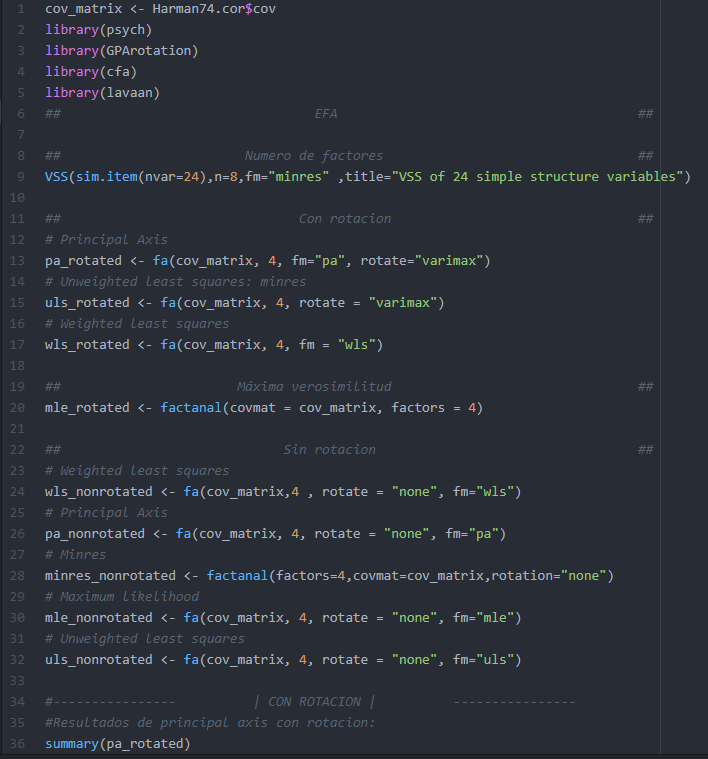
\includegraphics[scale=0.287]{./Imagenes/codigo1.png}
		\end{subfigure}
		\begin{subfigure}{0.49\textwidth}
			\centering
			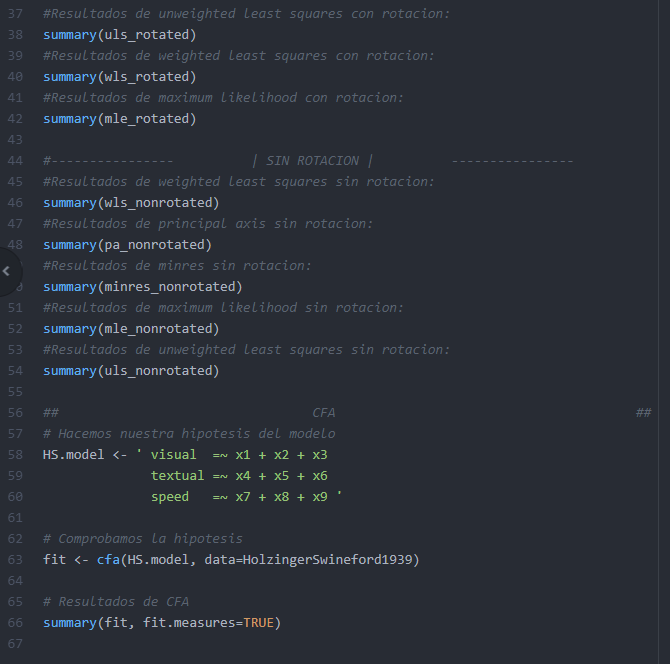
\includegraphics[scale=0.33]{./Imagenes/codigo2.png}
		\end{subfigure}
	\caption{Código de ejemplo en R}
	\end{figure}
\end{frame}

\begin{frame}[fragile]{Análisis de los resultados de fa}
	\metroset{block=fill}
	\begin{alertblock}{Resultados}
		Factor analysis with Call: fa(r = cov\_matrix, nfactors = 4, rotate = "varimax", fm = "pa")
		
		Test of the hypothesis that 4 factors are sufficient.
		The degrees of freedom for the model is 186  and the objective function was  1.72 
		
		The root mean square of the residuals (RMSA) is  0.04 
		The df corrected root mean square of the residuals is  0.05 
		
		\begin{itemize}
			\item La primera línea nos dice la llamada a la función fa.
			\item La segunda nos da la información sobre si los 4 factores son suficientes.
			\item La penúltima línea es la raíz cuadrada de la media de los residuos RMSA.
			\item La última línea es la raíz cuadrada de la media de los residuos estandarizados al cuadrado.
		\end{itemize}
	\end{alertblock}
\end{frame}

\begin{frame}[fragile]{Análisis de los resultados de fa}
\metroset{block=fill}
\begin{alertblock}{Resultados}
	Si hacemos una llamada con el objeto obtenido usando la función fa, por ejemplo pa\_rotate, obtenemos entre otras cosas una matriz de pesos que nos explica con qué pesos los factores explican cada variable de forma que podríamos poner cada variable menos su media como una combinación lineal de los factores con los pesos obtenidos.
\end{alertblock}
\end{frame}

\begin{frame}[fragile]{Análisis de los resultados de fa}
\metroset{block=fill}
\begin{alertblock}{Resultados}
	\begin{figure}
		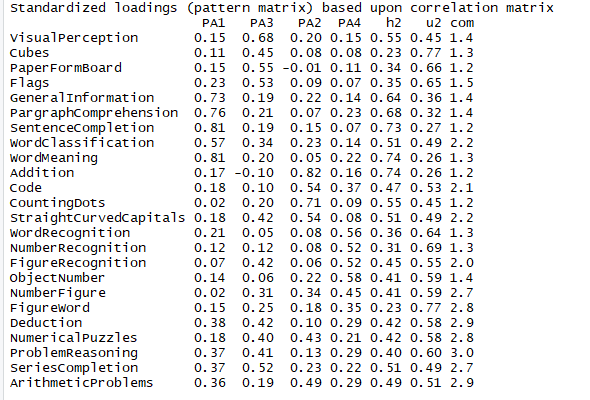
\includegraphics[scale=0.4]{./Imagenes/res_fa.png}
		\caption{Resultados del objeto fa}
	\end{figure}
	El valor h2 es la suma de todos los pesos al cuadrado para esa variable, u2 nos da una medida de la unicidad y com una medida de la complejidad para expresar esa variable con los factores obtenidos.
\end{alertblock}
\end{frame}

\begin{frame}[fragile]{Análisis de los resultados de VSS}
En este caso estamos llamando a la función VSS con unos datos simulados aleatorios de 24 variables.
\metroset{block=fill}
\begin{alertblock}{Resultados}
	\begin{figure}
		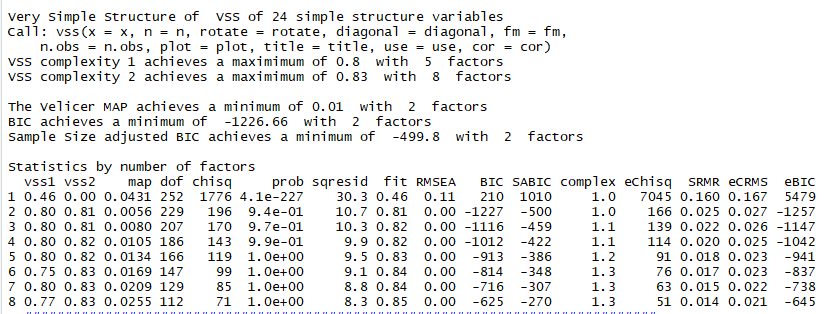
\includegraphics[scale=0.27]{./Imagenes/res_vss1.png}
		\caption{Resultados del objeto VSS}
	\end{figure}
	Podemos observar que con summary visualizamos todas las medidas de bonanza del modelo como por ejemplo con chisq (chi-cuadrado) tal y como explicamos en la etapa teórica. Además podemos observar que nos indica que el modelo con mejor ajuste y menor complejidad es el que tiene 2 factores.
\end{alertblock}
\end{frame}

\begin{frame}[fragile]{Análisis de los resultados de VSS}
Además podemos observar que la función hace un plot de la gráfica que compara la medida obtenida para cada tipo de medida y número de factores.
\metroset{block=fill}
\begin{alertblock}{Resultados}
	\begin{figure}
		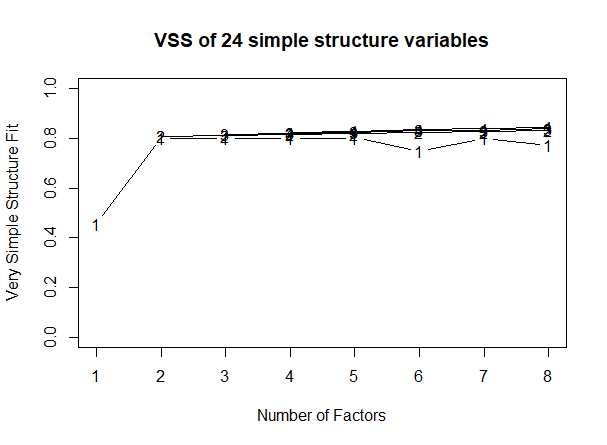
\includegraphics[scale=0.25]{./Imagenes/res_vss2.png}
		\caption{Resultados del plot de VSS}
	\end{figure}
	Como podemos observar el modelo obtiene una mejora al usar dos factores y no mejora al incrementar dicho número, por lo que los resultados obtenidos son consistentes.
\end{alertblock}
\end{frame}

\begin{frame}[fragile]{Análisis de los resultados de factanal}
\metroset{block=fill}
\begin{alertblock}{Resultados}
	Call:
	factanal(factors = 4, covmat = cov\_matrix)
	
	The degrees of freedom for the model is 186 and the fit was 1.7108 
	
	Nos arroja al igual que en fa una matriz con las combinaciones de los factores para explicar cada variable.
	
	Como podemos comprobar los resultados arrojados son iguales a los de la función fa, por lo que la interpretación es la misma.
\end{alertblock}
\end{frame}

\begin{frame}[fragile]{Análisis de los resultados de cfa}
En este caso estamos empleando el dataset HolzingerSwineford1939 compuesto por 9 variables que reflejan los patrones de respuestas de niños a unos tests. Se cree que el modelo puede ser explicado mediante 3 factores:
\begin{itemize}
	\item $visual = x_1 + x_2 + x_3$
	\item $textual = x_4 + x_5 + x_6$
	\item $celeridad = x_7 + x_8 + x_9$
\end{itemize}
De esta forma podemos expresas en R este modelo con sintaxis lavaan:
\begin{figure}
	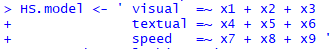
\includegraphics[scale=1]{./Imagenes/res_cfa1.png}
	\caption{Código para expresar el modelo}
\end{figure}
\end{frame}

\begin{frame}[fragile]{Análisis de los resultados de cfa}
\metroset{block=fill}
\begin{alertblock}{Resultados}
Si hacemos summary del objeto obtenido nos arroja la siguiente información:
\vspace{10px}
\begin{figure}
	\centering
	\begin{subfigure}{0.49\textwidth}
		\centering
		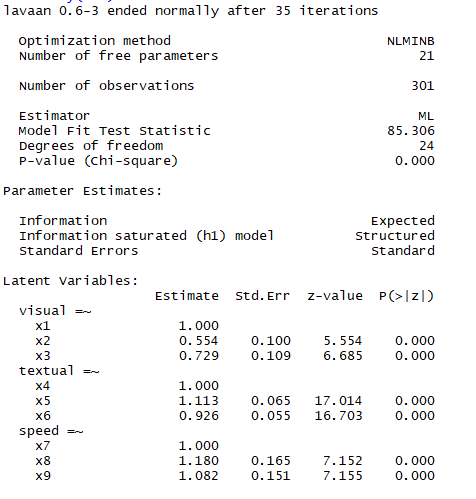
\includegraphics[scale=0.36]{./Imagenes/res_cfa_sum1.png}
	\end{subfigure}
	\begin{subfigure}{0.49\textwidth}
		\centering
		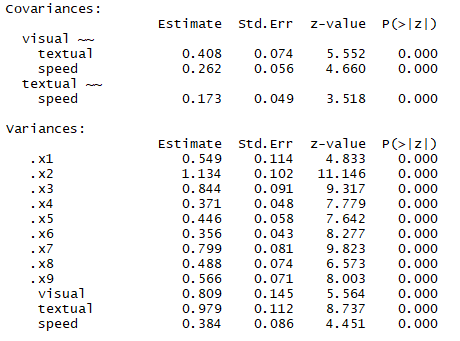
\includegraphics[scale=0.36]{./Imagenes/res_cfa_sum2.png}
	\end{subfigure}
	\caption{Resultados de summary(cfa)}
\end{figure}
\end{alertblock}
\end{frame}

\begin{frame}[fragile]{Análisis de los resultados de cfa}
Los resultados obtenidos son:
\metroset{block=fill}
\begin{alertblock}{Resultados}
	\begin{itemize}
		\item Si el método ha convergido y en cuantas iteraciones.
		\item El número de observaciones en los datos.
		\item Estimador usado, en este caso máxima verosimilitud.
		\item Valores estadísticos que nos miden entre otras cosas el error al usar los factores para explicar el modelo.
	\end{itemize}
\end{alertblock}
\end{frame}

\begin{frame}[standout]
	\LARGE{¿Preguntas?}
	\vspace{10px}
	\begin{figure}
		
\includegraphics[scale=0.5]{./Imagenes/preguntas.png}
	\end{figure}
\end{frame}


\end{document}
